\documentclass{article}
\newcommand{\docheader}{Results so far}
% Shared preamble of the BitSemCom + GRAND documents (Safaa's report template).
% Each document sets \docheader (the right-hand running head) before % Shared preamble of the BitSemCom + GRAND documents (Safaa's report template).
% Each document sets \docheader (the right-hand running head) before % Shared preamble of the BitSemCom + GRAND documents (Safaa's report template).
% Each document sets \docheader (the right-hand running head) before \input{preamble}.
\usepackage[utf8]{inputenc}
\usepackage[T1]{fontenc}
\usepackage{xcolor}
\usepackage{tcolorbox}
\usepackage{amsmath}
\usepackage{fancyhdr}
\usepackage{titlesec}
\usepackage{geometry}
\usepackage{sectsty}
\usepackage{tabularx}
\usepackage{mathptmx}
\usepackage{booktabs}
\usepackage{multirow}
\usepackage{graphicx}
\usepackage{enumitem}
\usepackage{amssymb}
\usepackage{colortbl}
\usepackage{longtable}
\usepackage{float}
\usepackage{hyperref}
\usepackage{listings}
\usepackage{tikz}
\usetikzlibrary{arrows.meta, positioning, calc, shapes.geometric, fit, backgrounds}

% Page layout
\geometry{margin=1in}

% Header and footer
\pagestyle{fancy}
\fancyhf{}
\fancyhead[L]{{BitSemCom + GRAND}}
\fancyhead[R]{\docheader}
\fancyfoot[C]{\thepage}

% Define colors
\definecolor{lightblue}{RGB}{240, 248, 255}
\definecolor{lightbeige}{RGB}{255, 250, 240}
\definecolor{lightpink}{RGB}{255, 230, 230}
\definecolor{deepred}{RGB}{128, 0, 0}
\definecolor{mygray}{RGB}{245, 245, 245}
\definecolor{darkblue}{RGB}{30, 60, 120}
\definecolor{lightgreen}{RGB}{232, 245, 233}
\definecolor{darkgreen}{RGB}{27, 94, 32}
\definecolor{codebg}{RGB}{245, 245, 245}
\definecolor{keyword}{RGB}{0, 0, 180}
\definecolor{sqlstring}{RGB}{163, 21, 21}
\definecolor{sqlcomment}{RGB}{0, 128, 0}

% Define subsubsubsection command
\setcounter{secnumdepth}{4}
\setcounter{tocdepth}{4}

% Title styling
\titleformat{\section}
  {\normalfont\Large\bfseries\color{deepred}}{\thesection}{1em}{}
\titleformat{\subsection}
  {\normalfont\Large\bfseries\color{deepred}}{\thesubsection}{1em}{}
\titleformat{\subsubsection}
  {\normalfont\large\bfseries\color{deepred}}{\thesubsubsection}{1em}{}
\titleformat{\paragraph}
  {\normalfont\normalsize\bfseries\color{deepred}}{\theparagraph}{1em}{}
\titleformat{\subparagraph}
  {\normalfont\normalsize\bfseries\color{deepred}}{\thesubparagraph}{1em}{}

\sectionfont{\color{deepred}}
\subsectionfont{\color{deepred}}
\subsubsectionfont{\color{deepred}}

% Reduce spacing
\titlespacing*{\section}{0pt}{10pt}{4pt}
\setlength{\parskip}{4pt}

% Important Note box
\newtcolorbox{importantnote}[1][]{
    colback=lightbeige, colframe=deepred, fonttitle=\bfseries, title=Important Note, sharp corners, boxrule=0.2mm, width=\textwidth, #1
}

% Box for each concept subsection
\newtcolorbox{conceptbox}[1][]{
    colback=lightblue, colframe=darkblue, fonttitle=\bfseries, boxrule=0.2mm, sharp corners, width=\textwidth, #1
}

% Box for findings
\newtcolorbox{findingbox}[2][]{
    colback=lightgreen, colframe=darkgreen, fonttitle=\bfseries, boxrule=0.2mm, sharp corners, width=\textwidth, title=#2, #1
}

% Warning box
\newtcolorbox{warningbox}[2][]{
    colback=lightpink, colframe=deepred, fonttitle=\bfseries, boxrule=0.2mm, sharp corners, width=\textwidth, title=#2, #1
}

% --- additions used by both documents ---
\hypersetup{hidelinks}
\graphicspath{{../figures/grand_review/}{../../results/figures/}}
\lstset{basicstyle=\ttfamily\small,breaklines=true,columns=fullflexible,keepspaces=true,
        backgroundcolor=\color{codebg},frame=single,framerule=0pt,xleftmargin=0.6em,xrightmargin=0.6em}
\newcommand{\file}[1]{\path{#1}}
\newcommand{\dB}{\,\mathrm{dB}}
\setlength{\tabcolsep}{4.5pt}
\setlength{\emergencystretch}{2em}
\setlist{nosep}
.
\usepackage[utf8]{inputenc}
\usepackage[T1]{fontenc}
\usepackage{xcolor}
\usepackage{tcolorbox}
\usepackage{amsmath}
\usepackage{fancyhdr}
\usepackage{titlesec}
\usepackage{geometry}
\usepackage{sectsty}
\usepackage{tabularx}
\usepackage{mathptmx}
\usepackage{booktabs}
\usepackage{multirow}
\usepackage{graphicx}
\usepackage{enumitem}
\usepackage{amssymb}
\usepackage{colortbl}
\usepackage{longtable}
\usepackage{float}
\usepackage{hyperref}
\usepackage{listings}
\usepackage{tikz}
\usetikzlibrary{arrows.meta, positioning, calc, shapes.geometric, fit, backgrounds}

% Page layout
\geometry{margin=1in}

% Header and footer
\pagestyle{fancy}
\fancyhf{}
\fancyhead[L]{{BitSemCom + GRAND}}
\fancyhead[R]{\docheader}
\fancyfoot[C]{\thepage}

% Define colors
\definecolor{lightblue}{RGB}{240, 248, 255}
\definecolor{lightbeige}{RGB}{255, 250, 240}
\definecolor{lightpink}{RGB}{255, 230, 230}
\definecolor{deepred}{RGB}{128, 0, 0}
\definecolor{mygray}{RGB}{245, 245, 245}
\definecolor{darkblue}{RGB}{30, 60, 120}
\definecolor{lightgreen}{RGB}{232, 245, 233}
\definecolor{darkgreen}{RGB}{27, 94, 32}
\definecolor{codebg}{RGB}{245, 245, 245}
\definecolor{keyword}{RGB}{0, 0, 180}
\definecolor{sqlstring}{RGB}{163, 21, 21}
\definecolor{sqlcomment}{RGB}{0, 128, 0}

% Define subsubsubsection command
\setcounter{secnumdepth}{4}
\setcounter{tocdepth}{4}

% Title styling
\titleformat{\section}
  {\normalfont\Large\bfseries\color{deepred}}{\thesection}{1em}{}
\titleformat{\subsection}
  {\normalfont\Large\bfseries\color{deepred}}{\thesubsection}{1em}{}
\titleformat{\subsubsection}
  {\normalfont\large\bfseries\color{deepred}}{\thesubsubsection}{1em}{}
\titleformat{\paragraph}
  {\normalfont\normalsize\bfseries\color{deepred}}{\theparagraph}{1em}{}
\titleformat{\subparagraph}
  {\normalfont\normalsize\bfseries\color{deepred}}{\thesubparagraph}{1em}{}

\sectionfont{\color{deepred}}
\subsectionfont{\color{deepred}}
\subsubsectionfont{\color{deepred}}

% Reduce spacing
\titlespacing*{\section}{0pt}{10pt}{4pt}
\setlength{\parskip}{4pt}

% Important Note box
\newtcolorbox{importantnote}[1][]{
    colback=lightbeige, colframe=deepred, fonttitle=\bfseries, title=Important Note, sharp corners, boxrule=0.2mm, width=\textwidth, #1
}

% Box for each concept subsection
\newtcolorbox{conceptbox}[1][]{
    colback=lightblue, colframe=darkblue, fonttitle=\bfseries, boxrule=0.2mm, sharp corners, width=\textwidth, #1
}

% Box for findings
\newtcolorbox{findingbox}[2][]{
    colback=lightgreen, colframe=darkgreen, fonttitle=\bfseries, boxrule=0.2mm, sharp corners, width=\textwidth, title=#2, #1
}

% Warning box
\newtcolorbox{warningbox}[2][]{
    colback=lightpink, colframe=deepred, fonttitle=\bfseries, boxrule=0.2mm, sharp corners, width=\textwidth, title=#2, #1
}

% --- additions used by both documents ---
\hypersetup{hidelinks}
\graphicspath{{../figures/grand_review/}{../../results/figures/}}
\lstset{basicstyle=\ttfamily\small,breaklines=true,columns=fullflexible,keepspaces=true,
        backgroundcolor=\color{codebg},frame=single,framerule=0pt,xleftmargin=0.6em,xrightmargin=0.6em}
\newcommand{\file}[1]{\path{#1}}
\newcommand{\dB}{\,\mathrm{dB}}
\setlength{\tabcolsep}{4.5pt}
\setlength{\emergencystretch}{2em}
\setlist{nosep}
.
\usepackage[utf8]{inputenc}
\usepackage[T1]{fontenc}
\usepackage{xcolor}
\usepackage{tcolorbox}
\usepackage{amsmath}
\usepackage{fancyhdr}
\usepackage{titlesec}
\usepackage{geometry}
\usepackage{sectsty}
\usepackage{tabularx}
\usepackage{mathptmx}
\usepackage{booktabs}
\usepackage{multirow}
\usepackage{graphicx}
\usepackage{enumitem}
\usepackage{amssymb}
\usepackage{colortbl}
\usepackage{longtable}
\usepackage{float}
\usepackage{hyperref}
\usepackage{listings}
\usepackage{tikz}
\usetikzlibrary{arrows.meta, positioning, calc, shapes.geometric, fit, backgrounds}

% Page layout
\geometry{margin=1in}

% Header and footer
\pagestyle{fancy}
\fancyhf{}
\fancyhead[L]{{BitSemCom + GRAND}}
\fancyhead[R]{\docheader}
\fancyfoot[C]{\thepage}

% Define colors
\definecolor{lightblue}{RGB}{240, 248, 255}
\definecolor{lightbeige}{RGB}{255, 250, 240}
\definecolor{lightpink}{RGB}{255, 230, 230}
\definecolor{deepred}{RGB}{128, 0, 0}
\definecolor{mygray}{RGB}{245, 245, 245}
\definecolor{darkblue}{RGB}{30, 60, 120}
\definecolor{lightgreen}{RGB}{232, 245, 233}
\definecolor{darkgreen}{RGB}{27, 94, 32}
\definecolor{codebg}{RGB}{245, 245, 245}
\definecolor{keyword}{RGB}{0, 0, 180}
\definecolor{sqlstring}{RGB}{163, 21, 21}
\definecolor{sqlcomment}{RGB}{0, 128, 0}

% Define subsubsubsection command
\setcounter{secnumdepth}{4}
\setcounter{tocdepth}{4}

% Title styling
\titleformat{\section}
  {\normalfont\Large\bfseries\color{deepred}}{\thesection}{1em}{}
\titleformat{\subsection}
  {\normalfont\Large\bfseries\color{deepred}}{\thesubsection}{1em}{}
\titleformat{\subsubsection}
  {\normalfont\large\bfseries\color{deepred}}{\thesubsubsection}{1em}{}
\titleformat{\paragraph}
  {\normalfont\normalsize\bfseries\color{deepred}}{\theparagraph}{1em}{}
\titleformat{\subparagraph}
  {\normalfont\normalsize\bfseries\color{deepred}}{\thesubparagraph}{1em}{}

\sectionfont{\color{deepred}}
\subsectionfont{\color{deepred}}
\subsubsectionfont{\color{deepred}}

% Reduce spacing
\titlespacing*{\section}{0pt}{10pt}{4pt}
\setlength{\parskip}{4pt}

% Important Note box
\newtcolorbox{importantnote}[1][]{
    colback=lightbeige, colframe=deepred, fonttitle=\bfseries, title=Important Note, sharp corners, boxrule=0.2mm, width=\textwidth, #1
}

% Box for each concept subsection
\newtcolorbox{conceptbox}[1][]{
    colback=lightblue, colframe=darkblue, fonttitle=\bfseries, boxrule=0.2mm, sharp corners, width=\textwidth, #1
}

% Box for findings
\newtcolorbox{findingbox}[2][]{
    colback=lightgreen, colframe=darkgreen, fonttitle=\bfseries, boxrule=0.2mm, sharp corners, width=\textwidth, title=#2, #1
}

% Warning box
\newtcolorbox{warningbox}[2][]{
    colback=lightpink, colframe=deepred, fonttitle=\bfseries, boxrule=0.2mm, sharp corners, width=\textwidth, title=#2, #1
}

% --- additions used by both documents ---
\hypersetup{hidelinks}
\graphicspath{{../figures/grand_review/}{../../results/figures/}}
\lstset{basicstyle=\ttfamily\small,breaklines=true,columns=fullflexible,keepspaces=true,
        backgroundcolor=\color{codebg},frame=single,framerule=0pt,xleftmargin=0.6em,xrightmargin=0.6em}
\newcommand{\file}[1]{\path{#1}}
\newcommand{\dB}{\,\mathrm{dB}}
\setlength{\tabcolsep}{4.5pt}
\setlength{\emergencystretch}{2em}
\setlist{nosep}


\begin{document}
\begin{center}
{\LARGE \bfseries \color{deepred} BitSemCom + GRAND}\\[2pt]
{\large \color{deepred} Results so far: does a channel code decoded with GRAND help a semantic image system?}\\[6pt]
{\normalsize Safaa Salman}\\[2pt]
{\small \emph{Thesis working document}, November 2026, branch \texttt{grand-implementation}}
\end{center}

\vspace{4pt}
\hrule
\vspace{8pt}

\begin{findingbox}{The answer in one paragraph}
Does an error-correcting code decoded with GRAND improve the image quality of a bit-level semantic
communication system? We measured it in two rounds on the BitSemCom models: first with the existing
checkpoints for $C=16$, 32 and 64 bits per token, then with a properly retrained $C=32$ model and a
model trained with GRAND inside the training loop, on AWGN and fading channels, with and without
channel-state errors, with four quality metrics. The answer is no: the CRC(128,112) code plus ORBGRAND
adds at most $+0.08\dB$ PSNR on AWGN, the gains seen in fading come from the interleaver and not from
the code, and the model trained with GRAND in the loop is 0.1 to 0.24 dB worse than the benchmark. The
reason is that the semantic decoder already absorbs scattered bit errors, so there is almost nothing
left for a code to repair. The one measurable win is for receivers that can only deliver hard bits. This
document explains the experiments and the numbers in plain language; the repository guide explains the
code.
\end{findingbox}

\tableofcontents

\section{The question and the short answer}

BitSemCom turns an image into a few thousand bits, sends them as QPSK symbols, and rebuilds the image
from the received \emph{soft values} (the probability that each bit is a 1). There is no channel code:
the semantic decoder is trained on noisy inputs and copes with bit errors by itself. The thesis asks
whether adding a code, decoded with GRAND, helps.

We added a CRC(128,112) code (16 parity bits per 112 data bits) with an interleaver between the bit
mapper and the decoder, decoded it with ORBGRAND, and compared image quality with and without it. When
ORBGRAND cannot decode a block within its guess budget it gives up (``abandons'') and the block is
passed on as plain soft values, exactly as without the code. So the code can only help where ORBGRAND
decodes, and can only hurt when it ``repairs'' a block to a wrong codeword (a \emph{miscorrection}).

\begin{findingbox}{Short answer}
The code plus GRAND does not improve image quality in any setting that matters:
\begin{itemize}
\item AWGN: at most $+0.08\dB$ PSNR (at 6 dB SNR); nothing or a small loss below 6 dB. The code
also spends 16\% more channel uses, worth about 0.2 dB if spent on more semantic bits instead.
\item Fading: the gains that look like GRAND's ($+0.06$ to $+0.26\dB$) come from the interleaver. The
same interleaver without the code does as well or better below 10 dB.
\item Training with GRAND in the loop: the resulting model is 0.09 to 0.24 dB worse than the benchmark
with every receiver, including with perfect bits. It is simply a worse autoencoder.
\item The one real win: receivers that can only deliver hard bits (0 or 1). There the code plus GRAND
gained $+0.1$ to $+0.4\dB$ in round 1.
\end{itemize}
\end{findingbox}

\section{What was measured and how}

\textbf{The system.} A $256\times256$ image becomes 256 tokens of $C$ bits each ($C=32$: 8192 bits).
Our coded link pads the bits to blocks of 112, adds 16 parity bits per block (CRC polynomial
\texttt{0x9eb2}, rate 0.875), interleaves, sends QPSK symbols through the channel, computes one LLR per
bit, and decodes each block with 1-line ORBGRAND. For $C=32$ that is 74 blocks and 4736 symbols instead
of 4096. The guess budget is 2000 in the main sweep (the budget used in training) and 100{,}000 in a
separate budget study.

\textbf{Models.} Round 1 used the existing stage-2 checkpoints for $C=16$, 32, 64 (fine-tuned on a noisy
channel with the original script, fixed learning rate, SNR $[-3,6]$ dB). Round 2 added two $C=32$
models trained with our trainer from the stage-2 checkpoint: \emph{bench} (30k steps, warmup + cosine
learning rate $10^{-4}\to10^{-6}$, SNR drawn per batch from $[0,10]$ dB) and \emph{grand} (the identical
recipe with CRC + ORBGRAND in the forward pass of every step, soft fallback).

\begin{table}[H]
\centering\footnotesize
\begin{tabular}{lllc}
\toprule
Model & Training & GRAND in the loop & PSNR with perfect bits (dB) \\
\midrule
stage2 & the old checkpoint, fixed learning rate & no & 23.46 \\
bench & 30k steps, warmup + cosine, SNR 0--10 dB & no & 24.22 \\
grand & identical recipe to bench & yes, budget 2000, soft fallback & 24.02 \\
\bottomrule
\end{tabular}
\caption{The three $C=32$ models of round 2.}
\end{table}

\textbf{Receivers.} Perfect bits (the ceiling); the plain BitSemCom soft receiver; the same with the
interleaver and no code; hard 0/1 decisions; the coded receiver (interleaver + CRC + ORBGRAND, soft
fallback). All receivers get the same bits and the same channel noise for a given image and SNR, so
every comparison is a \emph{paired} difference averaged over the 24 Kodak $256\times256$ crops, reported
with its standard error (s.e.) and the number of images on which the first receiver wins.

\textbf{Channels.} AWGN with perfect channel knowledge; AWGN where the receiver's SNR estimate is 3 dB
too high or too low; block Rayleigh fading with one gain per 8 QPSK symbols (16 bits, half a $C=32$ token); the same fading with a
channel-estimate error of variance 0.1. SNR ($E_s/N_0$ per symbol) from 0 to 12 dB.

\textbf{Metrics.} PSNR is the headline number (differences under about 0.03 dB are noise). MS-SSIM,
LPIPS and CLIP similarity were computed as well (section~\ref{sec:metrics}).

\section{Round 1: existing checkpoints, $C = 16$, 32, 64}

\subsection{AWGN}

Table~\ref{tab:r1awgn} shows PSNR for $C=16$; $C=32$ and 64 behave the same (see
\file{docs/grand_results.md}). The \emph{ceiling} is what a perfect channel would add (perfect bits
minus the plain receiver); the \emph{gain} is what the code added.

\begin{table}[H]
\centering\small
\begin{tabular}{ccccccc}
\toprule
$E_s/N_0$ (dB) & perfect bits & plain soft & hard 0/1 & coded soft & ceiling & gain \\
\midrule
2 & 22.25 & 21.69 & 21.32 & 21.29 & $+0.56$ & $-0.41$ \\
4 & 22.27 & 22.03 & 21.90 & 21.86 & $+0.24$ & $-0.17$ \\
5 & 22.24 & 22.08 & 21.98 & 22.04 & $+0.16$ & $-0.04$ \\
6 & 22.24 & 22.16 & 22.11 & 22.20 & $+0.08$ & $+0.04$ \\
7 & 22.25 & 22.20 & 22.18 & 22.25 & $+0.05$ & $+0.05$ \\
8 & 22.24 & 22.22 & 22.22 & 22.24 & $+0.02$ & $+0.02$ \\
10 & 22.26 & 22.26 & 22.26 & 22.26 & $0.00$ & $0.00$ \\
\bottomrule
\end{tabular}
\caption{Round 1, $C=16$, AWGN, CRC(128,112), budget 100{,}000, PSNR in dB over 24 patches.}
\label{tab:r1awgn}
\end{table}

Reading: where ORBGRAND works (from about 6 dB) the ceiling itself is under 0.1 dB, and the code
reaches it from 7 dB. Below 6 dB the code is harmful at this budget: 37 to 78\% of the blocks are
miscorrected into confidently wrong bits. Alternatives tried in round 1: a smaller budget caps the harm
but creates no gain; a stronger random linear code (128,104) with 24 parity bits removes the
miscorrections (never hurts, at most $+0.07\dB$) at 23\% overhead; a short CRC(64,48) gives the best
single number, $+0.13\dB$ at 5 dB, at 33\% overhead. At equal energy per semantic bit nothing beats the
plain receiver by more than 0.07 dB.

\textbf{Bandwidth.} Perfect-bit PSNR is 22.25 / 23.46 / 24.44 dB for $C=16$ / 32 / 64, about 1.1 dB per
doubling of the bits. The code's 14 to 16\% extra channel uses would therefore buy about 0.2 dB if spent
on semantic bits. Every coding gain measured is smaller than that.

\subsection{Why the gain is so small: diagnostics}

\begin{conceptbox}[title=Four facts about the semantic decoder]
\begin{itemize}
\item \textbf{The decoder tolerates about 5\% random bit noise.} The bit mapper is stochastic:
re-sampling it flips about 5\% of the bits and changes PSNR by nothing (22.23 vs 22.23 dB). The channel
at 6 dB flips 2.3\%.
\item \textbf{Scattered errors are cheap, clustered errors are expensive.} Flipping 2\% of the bits at
random costs 0.1 dB; wiping out 2\% of whole tokens costs 1.1 dB (table~\ref{tab:flips}). Which bits are
hit barely matters; concentration is what matters. A code fixes scattered errors, which the decoder does
not need; an interleaver breaks up clusters, which it does need.
\item \textbf{No channel of the bitstream is special.} Flipping 10\% of one channel's bits costs 0.03 to
0.06 dB for every one of the 16 channels, so unequal error protection has nothing to target.
\item \textbf{The SNR conditioning of the backbone is inert} in these checkpoints: telling the decoder
``the bits are clean'' after GRAND changes nothing.
\end{itemize}
\end{conceptbox}

\begin{table}[H]
\centering\small
\begin{tabular}{lcccc}
\toprule
flipped & random positions & most-confident bits & least-confident bits & whole tokens \\
\midrule
$C=16$, 1\% & 22.17 & 22.16 & 22.22 & 21.53 \\
$C=16$, 2\% & 22.12 & 22.09 & 22.21 & 21.16 \\
$C=16$, 5\% & 21.85 & 21.79 & 22.21 & 19.85 \\
$C=16$, 10\% & 21.36 & 20.84 & 22.17 & 18.01 \\
$C=64$, 2\% & 24.31 & 24.26 & 24.42 & 22.55 \\
$C=64$, 10\% & 23.47 & 22.57 & 24.40 & 17.98 \\
\bottomrule
\end{tabular}
\caption{PSNR (dB) after flipping a fraction of the bits in different ways; perfect bits give 22.23 ($C=16$) and 24.44 ($C=64$).}
\label{tab:flips}
\end{table}

\subsection{Block fading}

With one Rayleigh gain per token, a deep fade destroys a whole token: the plain receiver loses 0.6 dB
($C=16$) to 1.0 dB ($C=64$) at 6 dB average SNR. Interleaving alone, with no code, recovers most of
that ($+0.23$ to $+0.50\dB$ at 6 dB). Hard decisions are much worse than soft in fading ($-0.6$ to
$-1.1\dB$): faded bits arrive as probability 0.5 and the decoder treats them like erasures; a hard
decision throws that away. The code plus interleaver reaches the perfect-bit ceiling from about 14 dB
average SNR, $+0.06$ to $+0.07\dB$ above interleaving alone; at 6 to 10 dB it is below interleaving alone
because of miscorrections. Coding without interleaving is worse than doing nothing at every SNR.

\textbf{Hard-bit receivers.} Against a receiver that can only deliver 0/1 decisions, the code with
hard-decision fallback gained $+0.09\dB$ at 6 dB AWGN and $+0.36$ / $+0.23\dB$ at 6 / 10 dB in fading
($C=16$). This is the one setting where GRAND earns its place.

\section{Round 2: a proper benchmark and GRAND in the loop ($C = 32$)}

\subsection{Benchmark retraining}

The benchmark run raised the validation score (mean PSNR over 0, 3, 6 and 10 dB) from 23.07 to
23.65 dB in 30k steps (5.8 h on an L4 GPU). On the full evaluation it beats the old checkpoint by
$+0.27$ to $+0.75\dB$ on AWGN and $+0.14$ to $+0.69\dB$ in fading with the plain receiver, the gain
growing with SNR (figure~\ref{fig:training}). The one place it loses is the hard-decision receiver at
0 dB ($-0.35\dB$): the old model was trained down to $-3$ dB.

\begin{figure}[H]
\centering
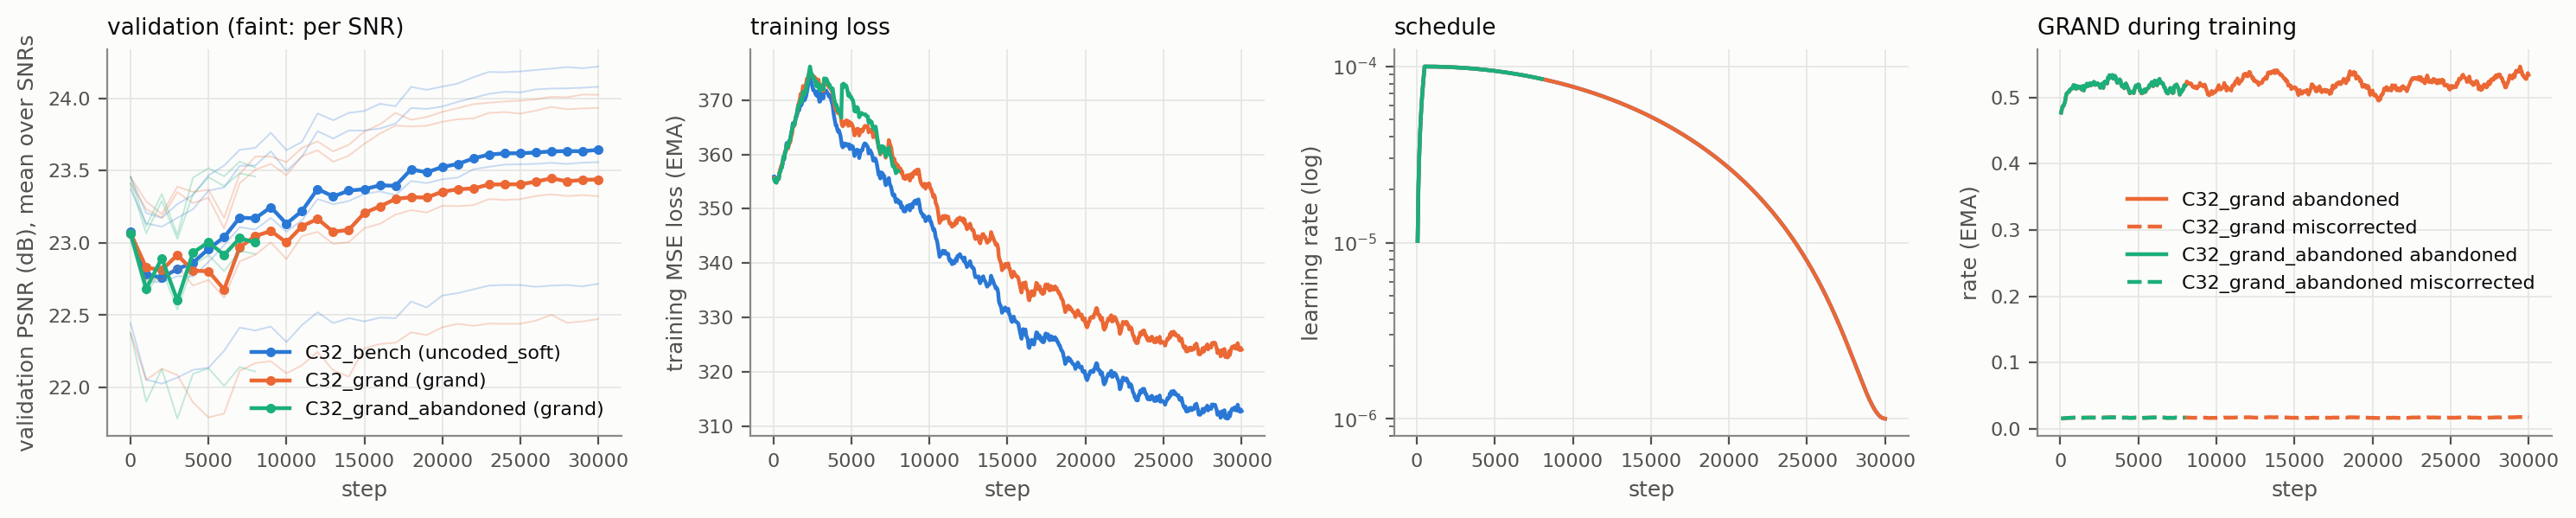
\includegraphics[width=\textwidth]{training.png}
\caption{Training curves of both runs: validation PSNR, training loss, learning-rate schedule and the
abandonment and miscorrection rates ORBGRAND reported inside the loop. Blue: benchmark. Orange: GRAND
in the loop (ends 0.2 dB lower). Green: a first GRAND attempt stopped at 8000 steps by early stopping.}
\label{fig:training}
\end{figure}

\subsection{Training with GRAND in the loop}

Same recipe, same starting weights; in every step the bits went through CRC encoding, the channel and
ORBGRAND (budget 2000, soft fallback) before the decoder. The gradient to the encoder was taken from the
uncoded soft channel, so both runs share one gradient path and differ only in the forward signal the
decoder sees.

\begin{table}[H]
\centering\footnotesize
\begin{tabular}{lcccccccc}
\toprule
Run & start & best score & at step & 0 dB & 3 dB & 6 dB & 10 dB & perfect bits \\
\midrule
bench (plain soft receiver) & 23.07 & 23.65 & 30{,}000 & 22.72 & 23.56 & 24.08 & 24.22 & 24.22 \\
grand (its own coded receiver) & 23.07 & 23.45 & 27{,}000 & 22.50 & 23.34 & 23.94 & 24.01 & 24.04 \\
\bottomrule
\end{tabular}
\caption{Validation PSNR (dB) on the 24 Kodak crops, AWGN; score = mean over the four SNRs.}
\end{table}

The GRAND-trained model is worse than bench with every receiver, in every condition: on AWGN by 0.09 dB
(0 dB) to 0.24 dB (4 dB) with its own coded receiver, by 0.17 to 0.22 dB with perfect bits, and by
0.16 to 0.23 dB with the plain soft receiver (s.e. 0.02 to 0.04); figure~\ref{fig:grandvsbench}. The
gap is the same with perfect bits as with the GRAND receiver, so this is a worse autoencoder, not a model
specialised to its decoder. Its coding gain equals bench's ($+0.10$ vs $+0.08\dB$ at 6 dB), so the
decoder did not learn to exploit ORBGRAND's output either. Inside the loop the GRAND statistics never
moved: about 50\% of blocks abandoned and 1.5\% miscorrected from step 50 to step 30{,}000, because with
fixed-power QPSK the encoder has no handle on which blocks decode. The training loss stayed about 3\%
above bench's for the whole run, which points at the gradient surrogate.

\begin{figure}[H]
\centering
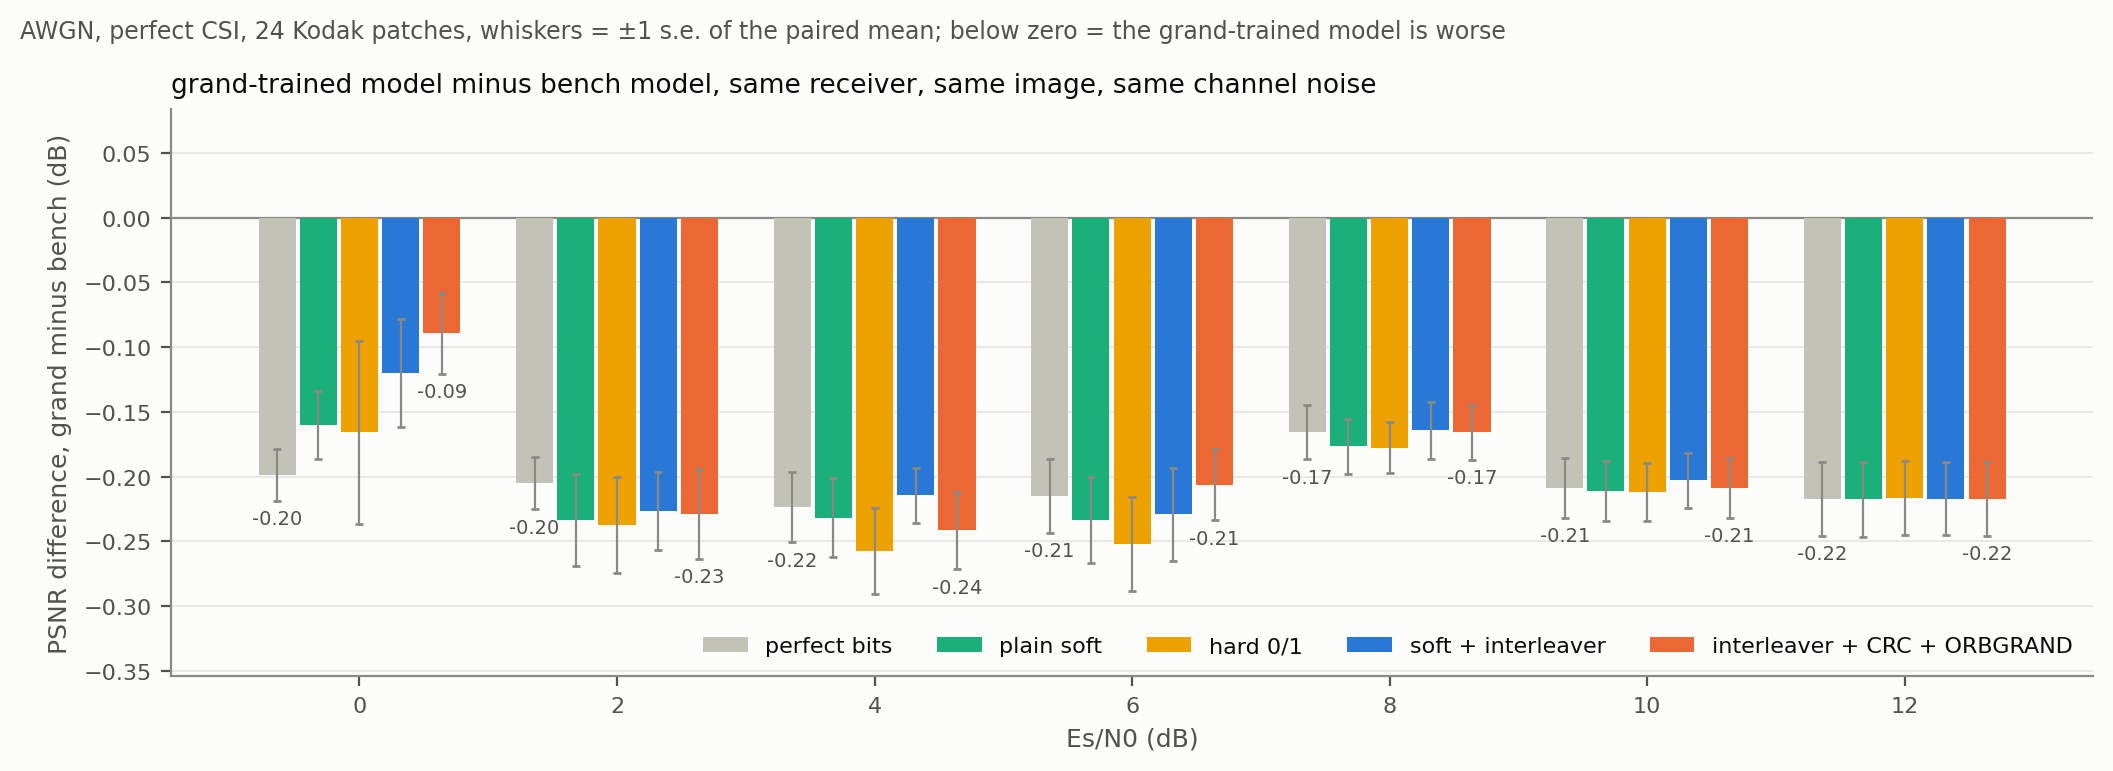
\includegraphics[width=\textwidth]{review_grand_vs_bench.png}
\caption{GRAND-trained model minus benchmark on AWGN, same receiver, same image, same noise. Every
bar is below zero, including with perfect bits (grey); the coded receiver (orange) is no closer to zero
than the others.}
\label{fig:grandvsbench}
\end{figure}

\subsection{The code at the receiver: AWGN}

\begin{figure}[H]
\centering
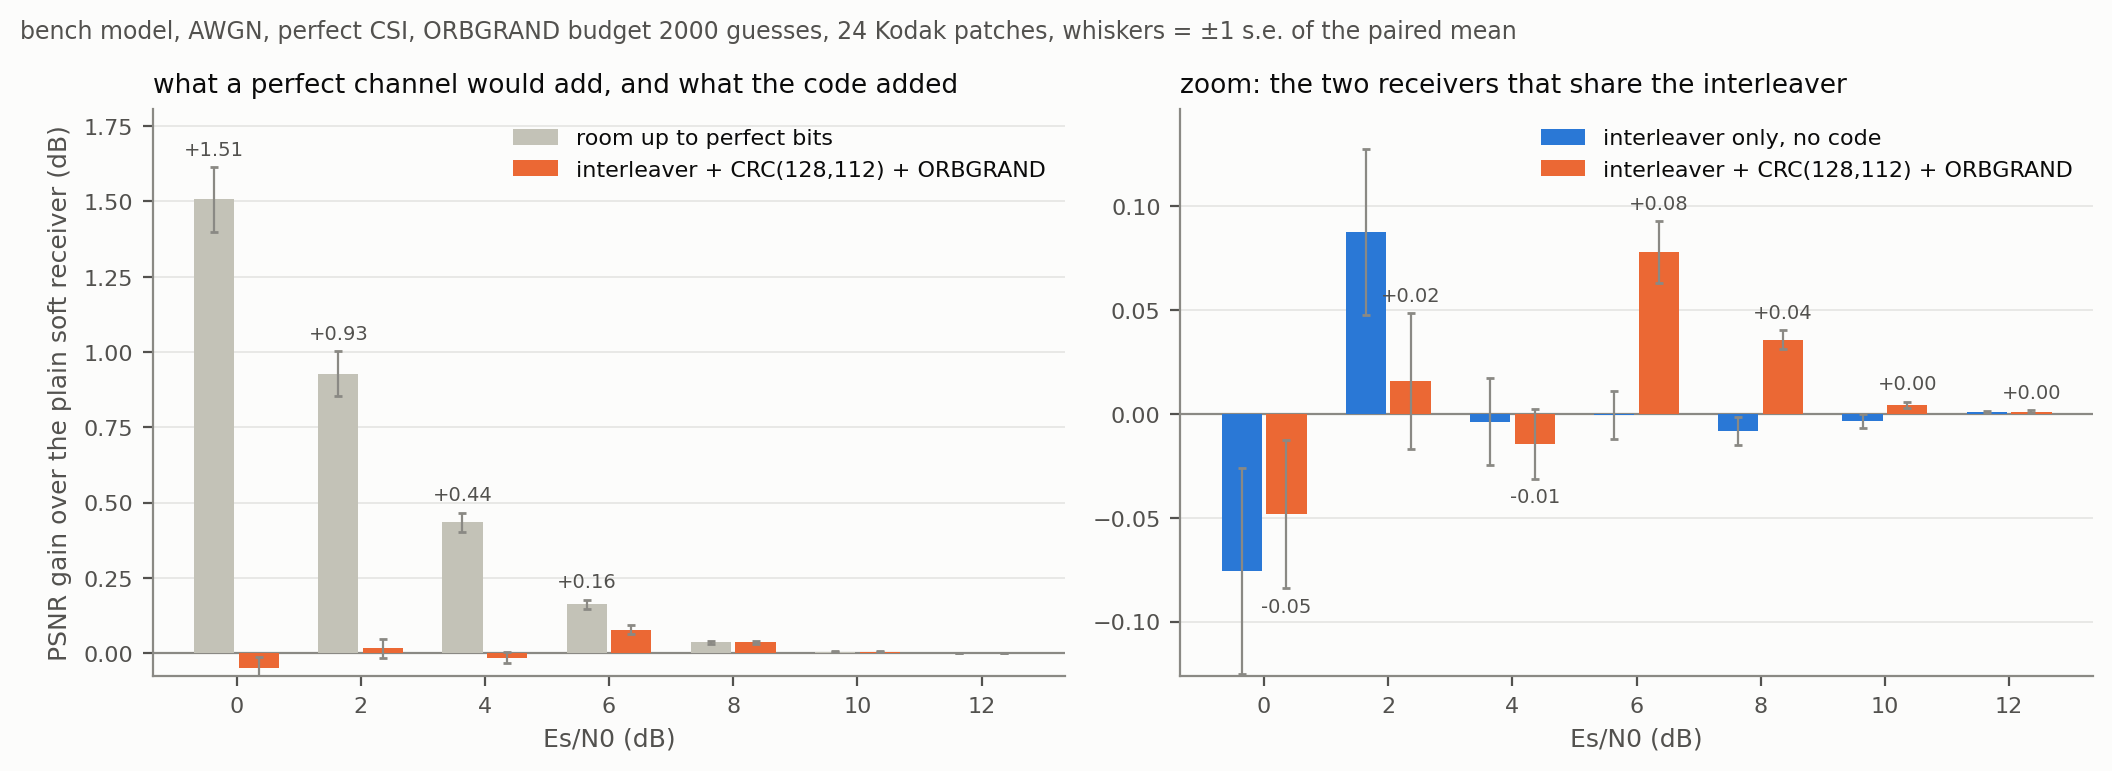
\includegraphics[width=\textwidth]{review_gain_awgn.png}
\caption{Bench model on AWGN. Left: how much PSNR is still available if every bit arrived correctly
(grey) next to what the code plus ORBGRAND gained (orange). Right: zoom on the two receivers that share
the interleaver. Whiskers are $\pm1$ s.e. of the paired mean over 24 images.}
\label{fig:gainawgn}
\end{figure}

\begin{table}[H]
\centering\footnotesize
\begin{tabular}{cccccccc}
\toprule
$E_s/N_0$ & perfect bits & plain soft & + interleaver & + code & code $-$ interleaver (wins) & abandoned & miscorrected \\
\midrule
0 & 24.21 & 22.70 & 22.63 & 22.66 & $+0.03\pm0.05$ (15/24) & 97.6\% & 2.4\% \\
2 & 24.23 & 23.30 & 23.39 & 23.31 & $-0.07\pm0.04$ (12/24) & 97.0\% & 3.0\% \\
4 & 24.23 & 23.79 & 23.79 & 23.78 & $-0.01\pm0.02$ (11/24) & 91.0\% & 3.0\% \\
6 & 24.23 & 24.07 & 24.07 & 24.15 & $+0.08\pm0.01$ (20/24) & 24.7\% & 0.7\% \\
8 & 24.22 & 24.18 & 24.17 & 24.22 & $+0.04\pm0.01$ (24/24) & 0.1\% & 0.0\% \\
10 & 24.21 & 24.21 & 24.21 & 24.21 & $+0.01\pm0.00$ (19/24) & 0\% & 0\% \\
12 & 24.22 & 24.22 & 24.22 & 24.22 & $0.00\pm0.00$ (13/24) & 0\% & 0\% \\
\bottomrule
\end{tabular}
\caption{Bench model, AWGN, PSNR in dB, budget 2000. ``Abandoned'' and ``miscorrected'' are fractions of the 74 blocks per image.}
\end{table}

Where ORBGRAND can decode (6 dB and up) the room up to perfect bits is 0.16 dB or less, and the code
recovers half of it at 6 dB and all of it at 8 dB. Below 6 dB the decoder gives up on 91 to 98\% of the
blocks and miscorrects 2 to 3\%, so the coded receiver is level with the plain one or slightly below.
The coded receiver wins on 20 of 24 images at 6 dB and 24 of 24 at 8 dB, but by 0.08 and 0.04 dB.
Figure~\ref{fig:example} shows that the difference is invisible.

\begin{figure}[H]
\centering
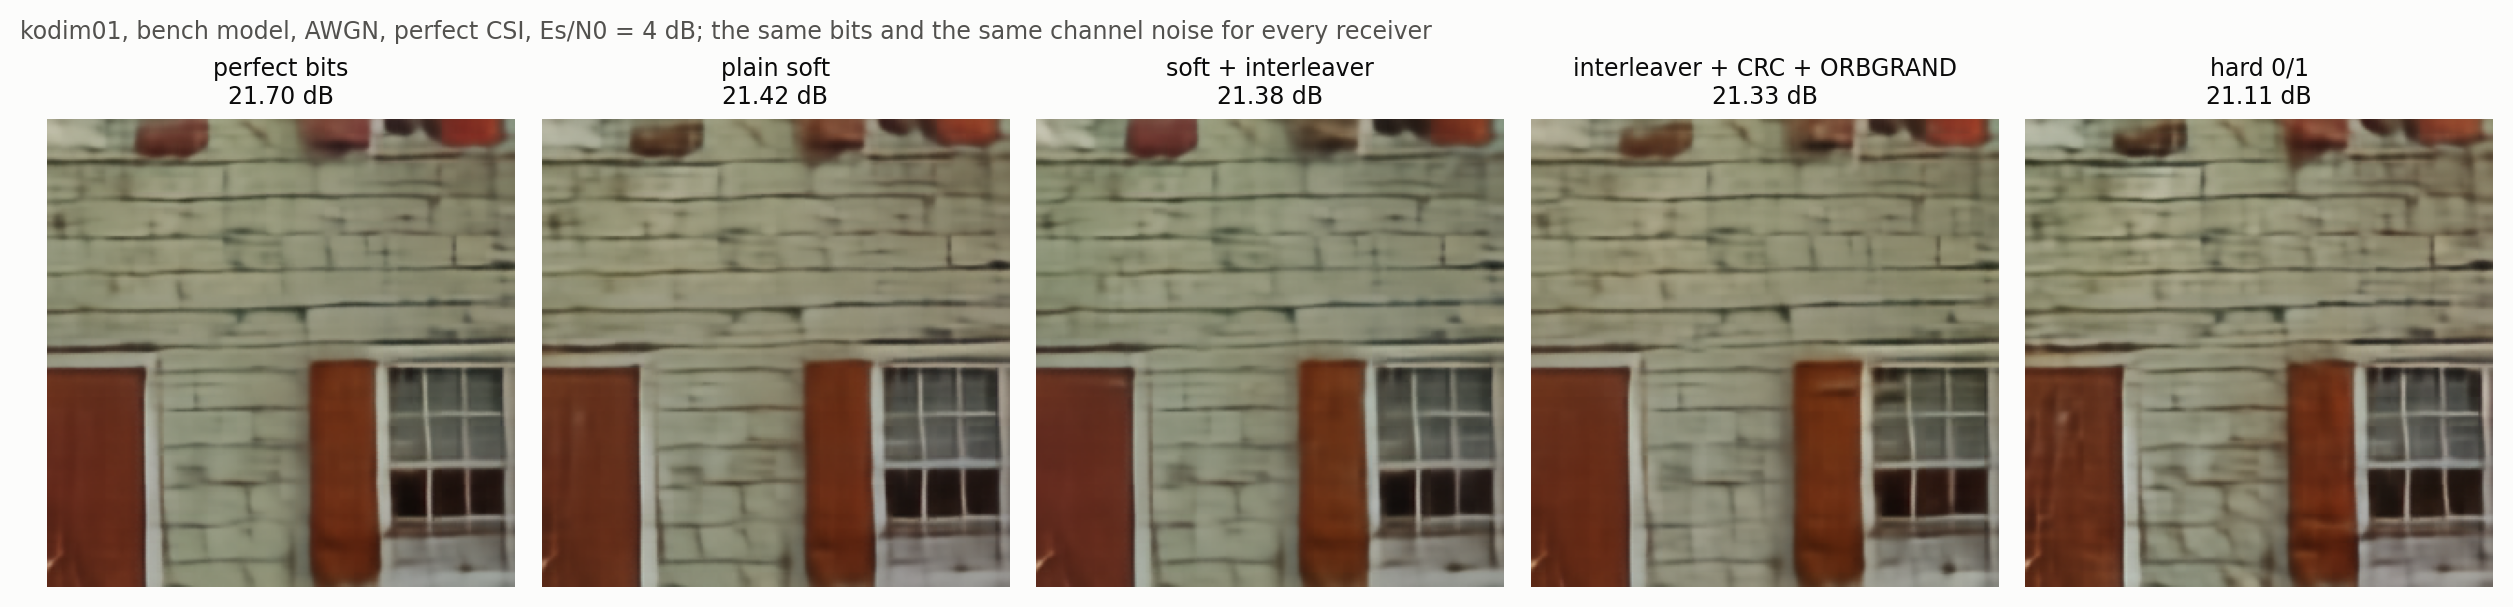
\includegraphics[width=\textwidth]{review_example_kodim01_awgn_4dB.png}
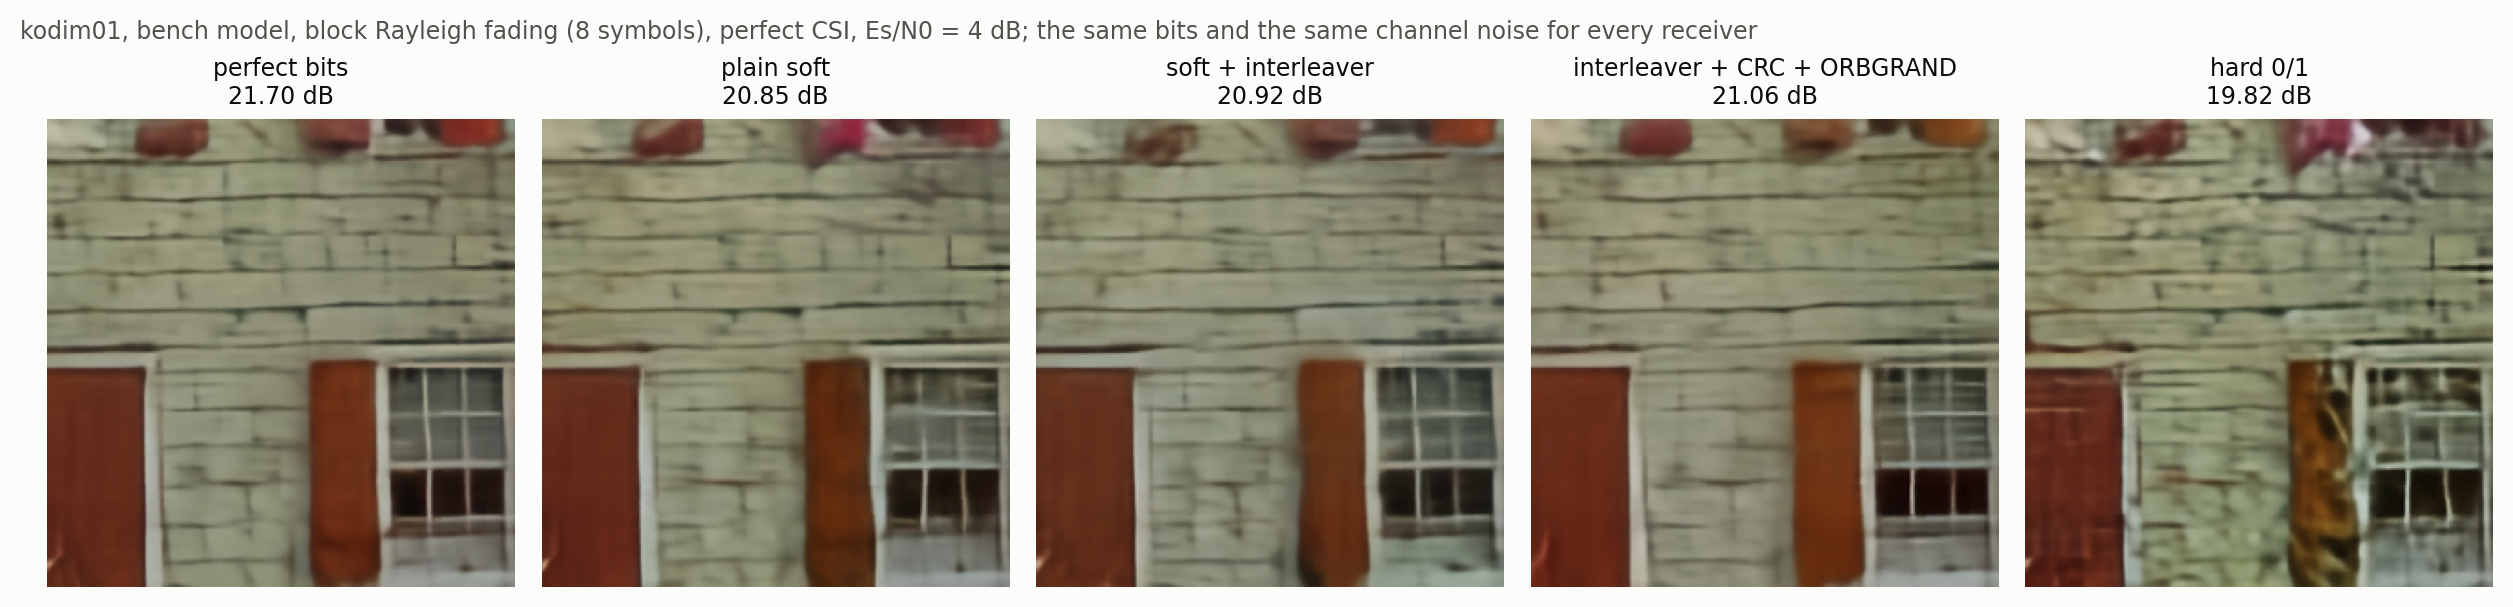
\includegraphics[width=\textwidth]{review_example_kodim01_fade8_4dB.png}
\caption{One patch at 4 dB, same bits and same noise for every receiver. Top: AWGN, the four
soft-input receivers are indistinguishable. Bottom: block fading, the interleaved receivers are 0.1 to
0.2 dB above the plain one and the hard-decision receiver shows the damage of whole faded tokens.}
\label{fig:example}
\end{figure}

\subsection{The code at the receiver: block fading}

\begin{figure}[H]
\centering
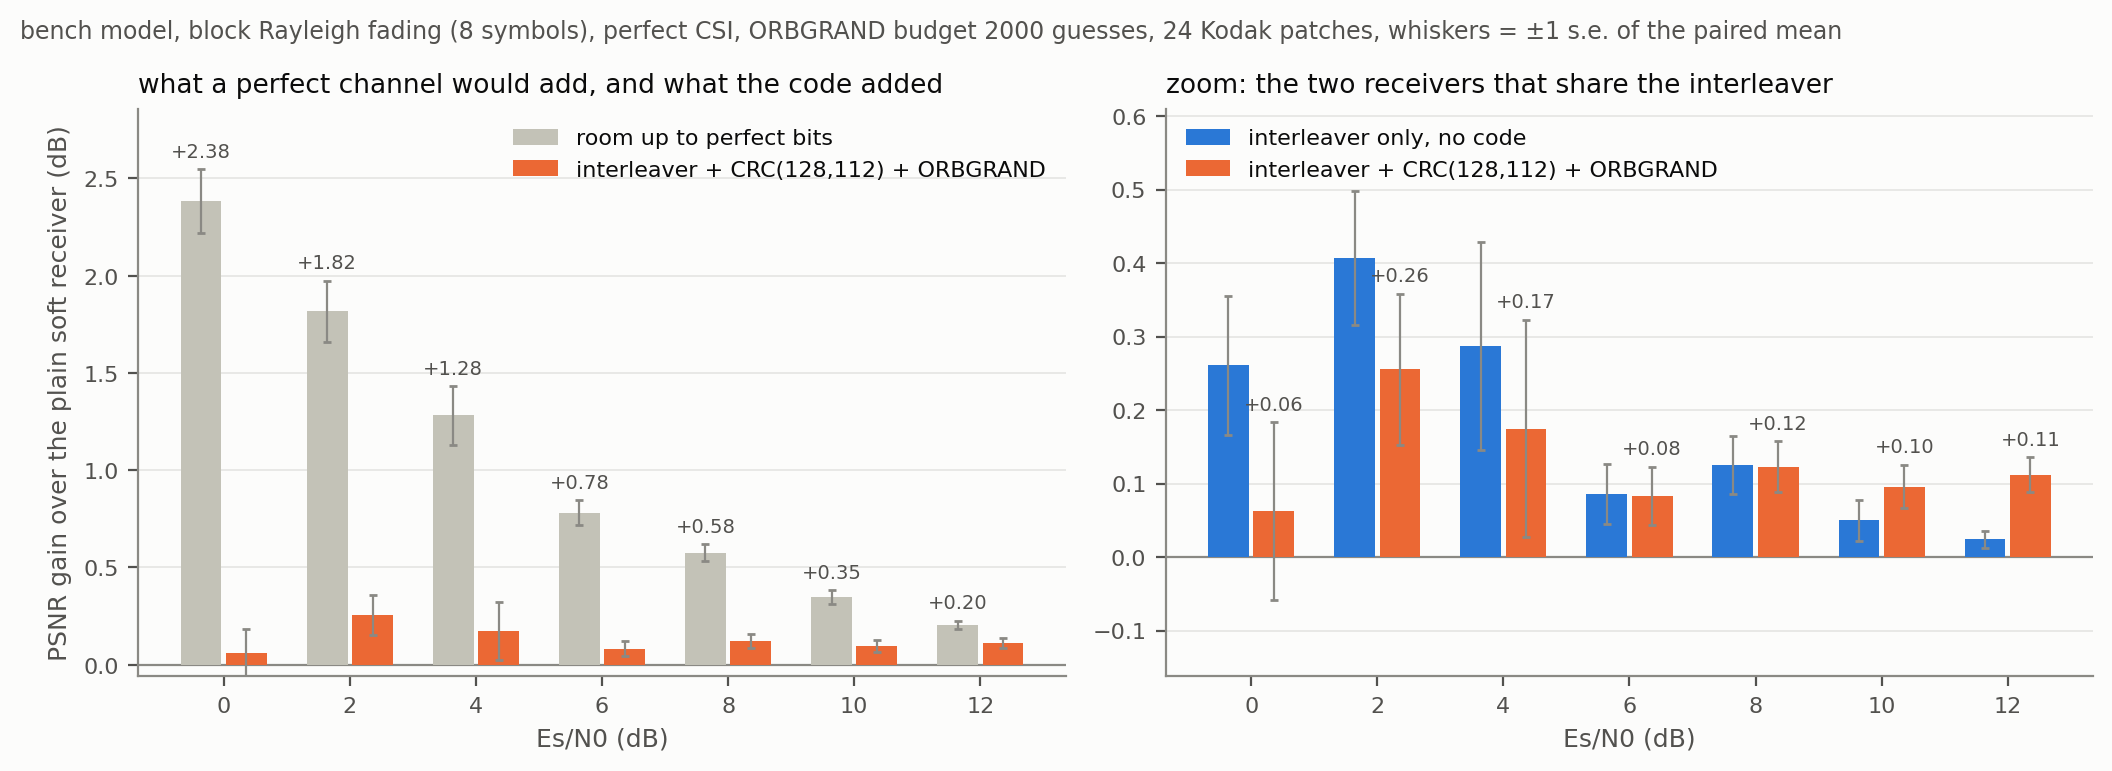
\includegraphics[width=\textwidth]{review_gain_fade8.png}
\caption{Bench model in block Rayleigh fading (one fade per 8 symbols). Left: room up to perfect bits
(grey) against the coded gain (orange). Right: the interleaver alone (blue) against the interleaver plus
code (orange), both measured against the plain receiver.}
\label{fig:gainfade}
\end{figure}

\begin{table}[H]
\centering\footnotesize
\begin{tabular}{cccccccc}
\toprule
$E_s/N_0$ & perfect bits & plain soft & + interleaver & + code & code $-$ interleaver (wins) & abandoned & miscorrected \\
\midrule
0 & 24.21 & 21.83 & 22.09 & 21.89 & $-0.20\pm0.07$ (6/24) & 96.7\% & 3.3\% \\
2 & 24.23 & 22.41 & 22.82 & 22.67 & $-0.15\pm0.05$ (5/24) & 96.4\% & 3.6\% \\
4 & 24.23 & 22.95 & 23.23 & 23.12 & $-0.11\pm0.06$ (10/24) & 97.2\% & 2.8\% \\
6 & 24.23 & 23.45 & 23.54 & 23.54 & $0.00\pm0.05$ (11/24) & 96.3\% & 3.4\% \\
8 & 24.22 & 23.64 & 23.77 & 23.77 & $0.00\pm0.03$ (12/24) & 93.5\% & 2.8\% \\
10 & 24.21 & 23.87 & 23.92 & 23.96 & $+0.05\pm0.02$ (17/24) & 68.1\% & 2.4\% \\
12 & 24.22 & 24.02 & 24.04 & 24.13 & $+0.09\pm0.02$ (20/24) & 31.6\% & 1.2\% \\
\bottomrule
\end{tabular}
\caption{Bench model, block Rayleigh fading (8 symbols per fade), PSNR in dB, budget 2000.}
\end{table}

In fading the plain receiver loses up to 2.4 dB because a deep fade wipes out whole tokens. The
interleaver alone recovers $+0.26$ / $+0.41$ / $+0.29\dB$ at 0 / 2 / 4 dB by spreading those errors over
the image. The coded receiver uses the same interleaver and sits below it at 0 to 4 dB (miscorrections)
and level with it at 6 to 8 dB. Only from 10 dB, where abandonment falls from 97\% to 68\% and then
32\%, does the code add $+0.05$ to $+0.09\dB$ on top of the interleaver. Against the plain receiver the
coded numbers read $+0.06$ to $+0.26\dB$: that is the interleaver, not the code.

\subsection{Hard-decision receivers}

\begin{table}[H]
\centering\small
\begin{tabular}{lcccc}
\toprule
Receiver & AWGN 0 dB & AWGN 6 dB & fading 0 dB & fading 6 dB \\
\midrule
plain soft & 22.70 & 24.07 & 21.83 & 23.45 \\
hard 0/1 & 21.03 & 23.94 & 19.13 & 22.45 \\
interleaver + code, soft fallback & 22.66 & 24.15 & 21.89 & 23.54 \\
\bottomrule
\end{tabular}
\caption{Bench model, PSNR in dB.}
\end{table}

\begin{importantnote}[title=A number to quote carefully]
Hard decisions cost 1.7 dB at 0 dB AWGN and 2.7 dB at 0 dB fading. The soft-fallback coded receiver
beats the hard receiver by the same amounts, but that measures soft versus hard input, not GRAND: at
0 dB 97\% of the blocks are abandoned and arrive as soft values. The honest hard-bit number is the round-1
comparison of the code \emph{with hard fallback} against hard decisions: $+0.09\dB$ at 6 dB AWGN,
$+0.36$ and $+0.23\dB$ at 6 and 10 dB in fading.
\end{importantnote}

\subsection{Imperfect channel knowledge}

\begin{figure}[H]
\centering
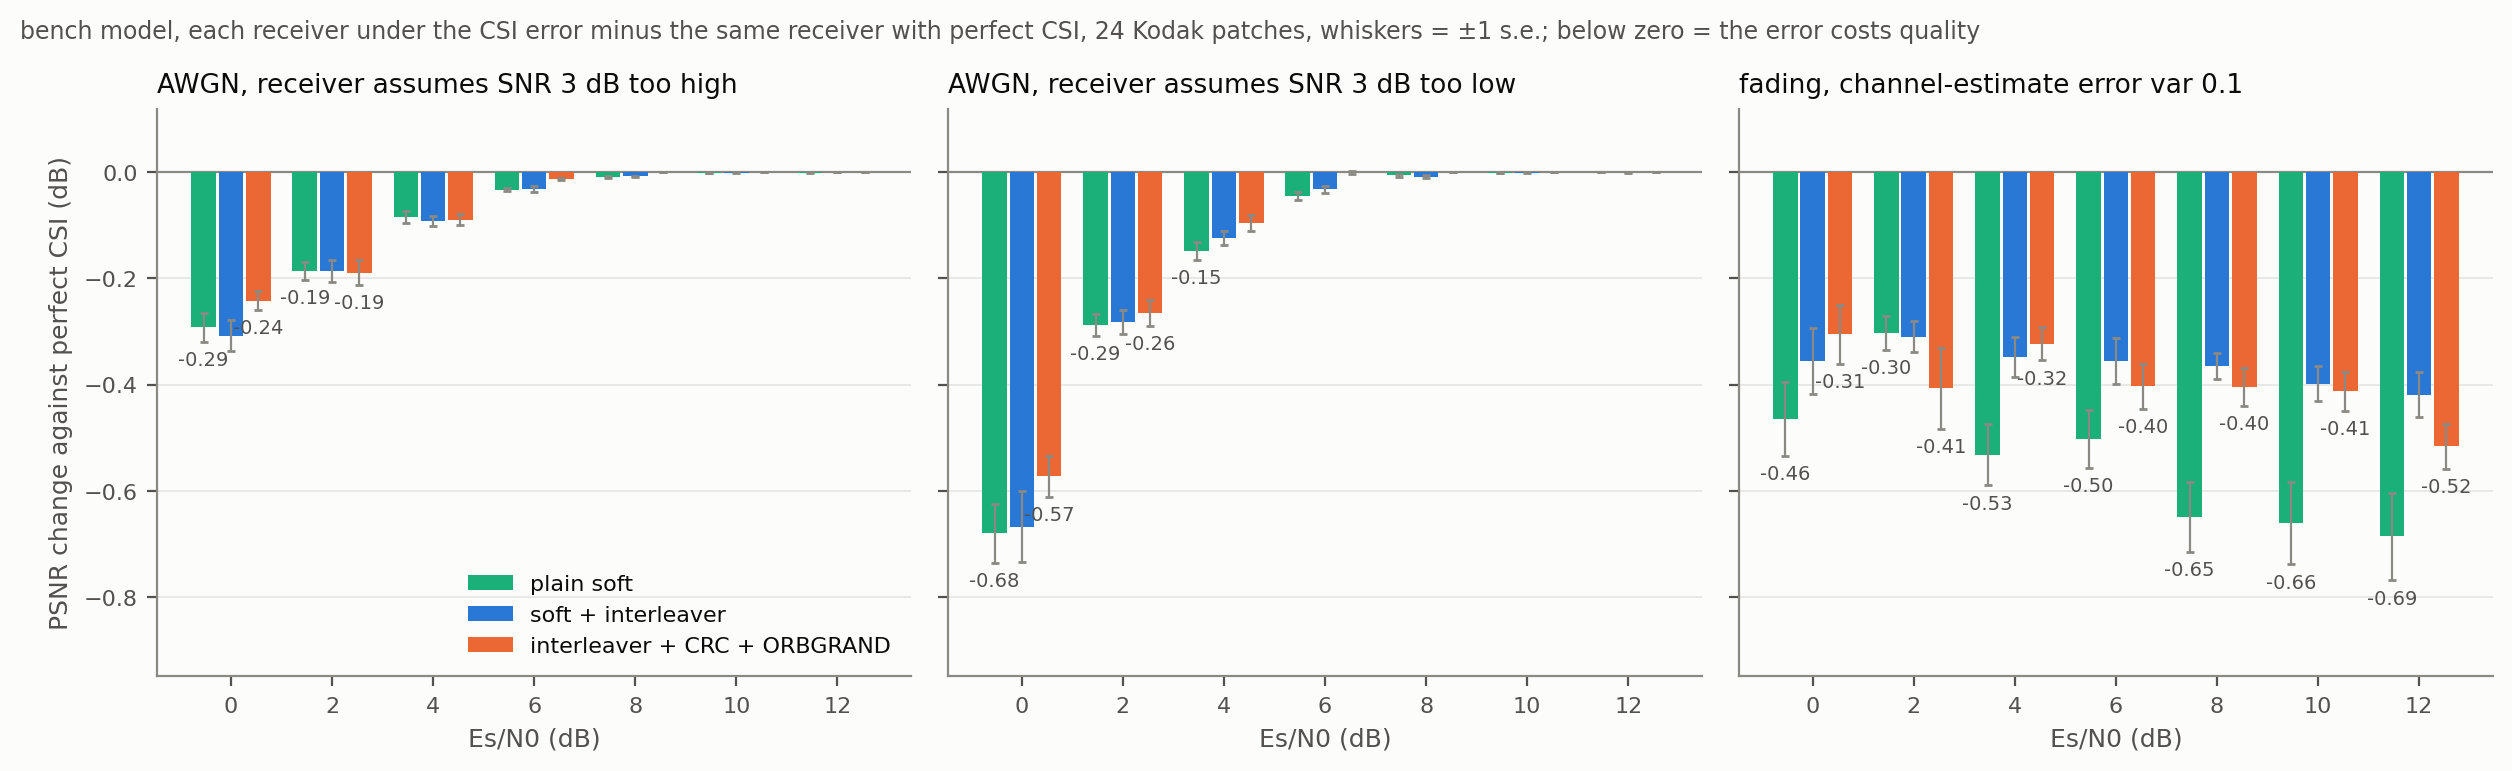
\includegraphics[width=\textwidth]{review_csi.png}
\caption{PSNR change of each receiver under a channel-state error, against the same receiver with
perfect knowledge (bench model; below zero = the error costs quality).}
\label{fig:csi}
\end{figure}

An SNR over-estimate of 3 dB costs the plain receiver 0.29 dB at 0 dB and nothing from 8 dB on; an
under-estimate costs 0.68 dB at 0 dB, 0.29 at 2 dB, 0.15 at 4 dB. The coded receiver pays almost the
same below 6 dB (0.24 and 0.57 dB at 0 dB) because its abandoned blocks fall back to the same
miscalibrated soft values, and nothing from 6 dB on. A channel-estimate error of variance 0.1 in fading
costs the plain receiver 0.46 to 0.69 dB, growing with SNR, the interleaved receiver 0.31 to 0.42 dB,
and the coded receiver 0.31 to 0.52 dB; with that error the block failure rate stays at 94 to 98\% up to
12 dB, so the code never decodes and never beats the interleaver alone.

ORBGRAND itself is immune to an SNR misestimate: its guessing order depends only on the ranking of the
LLRs, which a scale error does not change (section~\ref{sec:llr}). This does not show in image quality
because the coded receiver's quality below 6 dB is set by its abandoned blocks, which are soft values.

\subsection{Guess budget: 2000 against 100{,}000}

\begin{figure}[H]
\centering
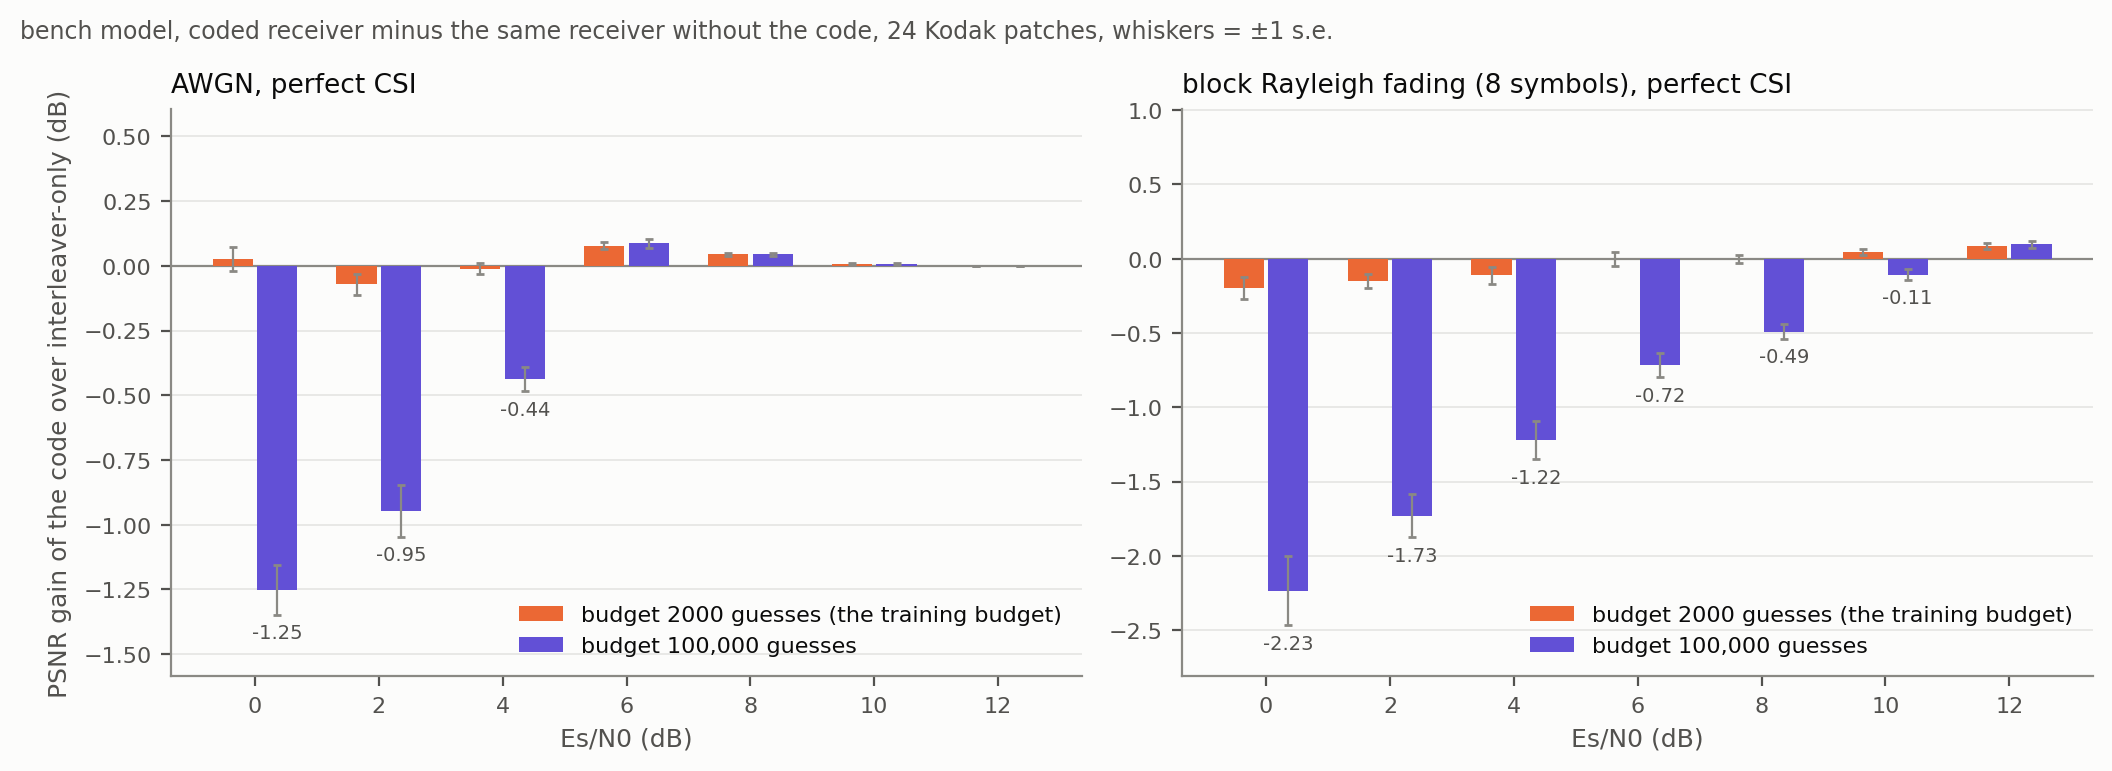
\includegraphics[width=\textwidth]{review_budget.png}
\caption{Gain of the code over the interleaver-only receiver at the two budgets, bench model.}
\end{figure}

A larger budget turns abandoned blocks into miscorrected ones. Below 6 dB AWGN and below 10 dB fading,
67 to 81\% of the blocks come back as confidently wrong codewords and the coded receiver loses 0.4 to
1.3 dB (AWGN) and 0.5 to 2.2 dB (fading). Where the code works (6 to 8 dB AWGN, 12 dB fading) the two
budgets give the same gain. With 16 parity bits the code is too weak for the error rates below 6 dB;
the budget only decides whether a failed block is declared (abandonment, harmless) or hidden
(miscorrection, harmful).

\subsection{Metrics beyond PSNR}
\label{sec:metrics}

\begin{table}[H]
\centering\small
\begin{tabular}{lcccc}
\toprule
Condition, $E_s/N_0$ & PSNR (dB) & MS-SSIM & LPIPS (lower is better) & CLIP similarity \\
\midrule
AWGN 6 dB & $+0.078\pm0.013$ & $+0.004\pm0.001$ & $-0.003\pm0.001$ & $-0.007\pm0.004$ \\
AWGN 8 dB & $+0.044\pm0.006$ & $+0.002\pm0.000$ & $-0.002\pm0.001$ & $-0.001\pm0.001$ \\
fading 0 dB & $-0.198\pm0.074$ & $-0.005\pm0.003$ & $+0.005\pm0.004$ & $-0.005\pm0.010$ \\
fading 2 dB & $-0.152\pm0.046$ & $-0.009\pm0.002$ & $-0.002\pm0.004$ & $+0.007\pm0.010$ \\
fading 12 dB & $+0.088\pm0.020$ & $+0.003\pm0.001$ & $-0.004\pm0.001$ & $+0.003\pm0.004$ \\
\bottomrule
\end{tabular}
\caption{Bench model, coded receiver minus interleaver-only receiver, paired over 24 images, $\pm1$ s.e.}
\end{table}

MS-SSIM and LPIPS agree with PSNR in sign wherever PSNR moves by more than 0.03 dB; the exceptions are
inside their standard errors. CLIP similarity differences sit inside a standard error of about 0.01
everywhere: 24 images are too few for it. The ordering of receivers is the same under PSNR, MS-SSIM and
LPIPS, so none of the new metrics changes the conclusion. For the thesis we suggest PSNR plus LPIPS,
with CLIP only on a few hundred images.

\subsection{The LLR study}
\label{sec:llr}

\begin{figure}[H]
\centering
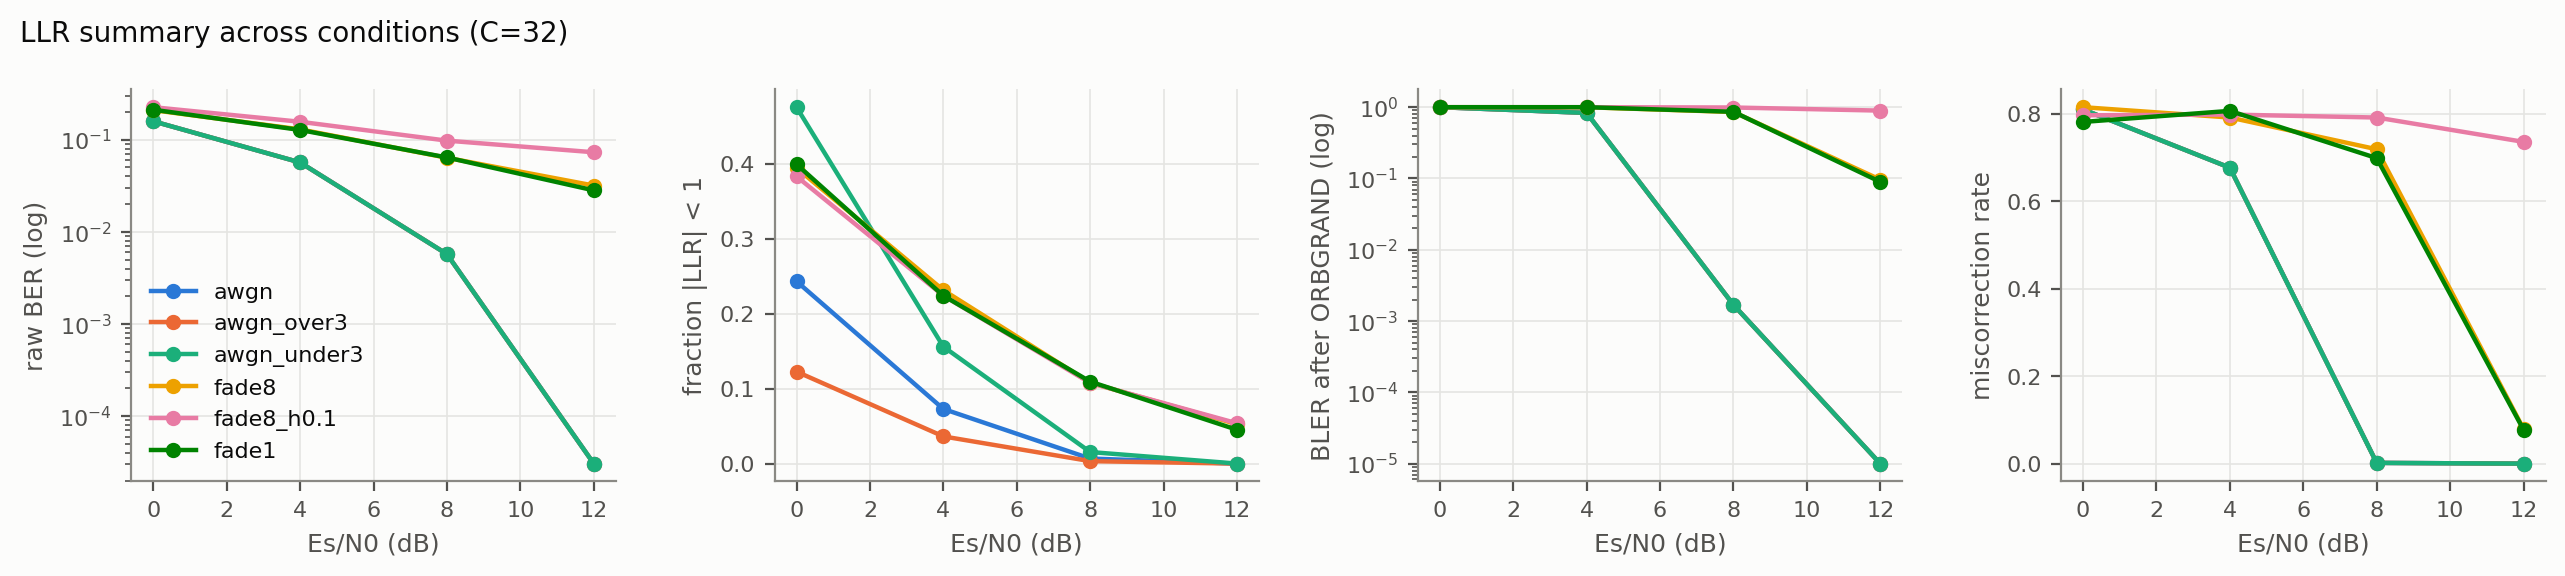
\includegraphics[width=\textwidth]{llr_summary.png}
\caption{Raw bit error rate, fraction of weak LLRs ($|\mathrm{LLR}|<1$), block error rate after ORBGRAND
and miscorrection rate per condition, stage2 model, large guess budget. The three AWGN curves lie on top
of each other in every panel except the second.}
\end{figure}

\begin{table}[H]
\centering\footnotesize
\begin{tabular}{p{4.4cm}ccccc}
\toprule
Condition & $E_s/N_0$ & raw BER & mean $|\mathrm{LLR}|$ & fraction $|\mathrm{LLR}|<1$ & BLER after GRAND \\
\midrule
AWGN, perfect CSI & 0 & 0.159 & 2.3 & 0.24 & 1.00 \\
AWGN, SNR assumed 3 dB too high & 0 & 0.159 & 4.7 & 0.12 & 1.00 \\
AWGN, SNR assumed 3 dB too low & 0 & 0.159 & 1.2 & 0.48 & 1.00 \\
AWGN, perfect CSI & 8 & 0.0057 & 12.6 & 0.007 & 0.0017 \\
AWGN, SNR assumed 3 dB too high & 8 & 0.0057 & 25.2 & 0.003 & 0.0017 \\
AWGN, SNR assumed 3 dB too low & 8 & 0.0057 & 6.3 & 0.016 & 0.0017 \\
block fading, perfect CSI & 12 & 0.032 & 30.5 & 0.053 & 0.096 \\
block fading, channel-estimate error 0.1 & 12 & 0.073 & 30.8 & 0.054 & 0.895 \\
\bottomrule
\end{tabular}
\caption{The LLR study in numbers.}
\end{table}

Two mechanisms. An SNR misestimate rescales the LLRs and changes the fraction of near-erasures the soft
decoder sees, but leaves their ranking untouched, so ORBGRAND's decisions are identical in the three
cases. A channel-estimate error in fading is different in kind: it raises the raw bit error rate from
3.2\% to 7.3\% at 12 dB, and 16 parity bits cannot absorb that, so block failures go from 10\% to 90\%.
This is the mechanism behind ``GRAND looks bad on bad channels'': the code is too weak for the error
rate, not the decoder.

\subsection{The MATLAB reference check}

\begin{warningbox}{Open item: the bit-exact check}
The decoder used everywhere is our Python port of Ken Duffy's ORBGRAND. It reproduced the block error
rates published with GRAND-MATLAB in round 1, and a test set of 740 real LLR blocks is exported for a
bit-exact comparison with the unmodified MATLAB functions. That comparison has not been run yet: it
needs a MATLAB session, and the Octave attempt failed on a MATLAB-only \texttt{cumsum} option.
\end{warningbox}

\section{What the results mean}

The semantic decoder was trained to live with noisy bits, so a channel code has very little left to
fix. Where GRAND works (from about 6 dB with 16 parity bits) the room up to perfect bits is under 0.2 dB
and the code recovers it, which is all of almost nothing. Below 6 dB the code is too weak: blocks are
abandoned (no change) or miscorrected (harm), and a bigger budget only converts the first into the
second. Soft values act as erasures, so any receiver that keeps them keeps most of the robustness, code
or no code. The 16\% extra bandwidth would buy about 0.2 dB as semantic bits, more than any coding gain
measured. And training with GRAND in the loop cannot help through the encoder, which has no handle on
block decodability; in our run it did not help through the decoder either.

For the thesis this is a clean negative result with a mechanism behind it: for a bit-level semantic
system with a soft-input decoder, a high-rate code plus GRAND does not improve image quality on AWGN or
fading channels, because the decoder already absorbs scattered bit errors and the interleaver handles
clustered ones.

\begin{findingbox}{Three framings with evidence behind them}
\begin{enumerate}
\item GRAND for receivers that only deliver hard bits ($+0.1$ to $+0.4\dB$ in round 1), a realistic
deployment constraint.
\item Interleaving first, with the code reaching the perfect-bit ceiling from about 10 to 14 dB
average SNR in fading, for bit-exact delivery.
\item GRAND's immunity to SNR misestimates (its guessing order depends only on LLR ranking), which only
pays off where GRAND actually decodes.
\end{enumerate}
\end{findingbox}

\section{Open items and next steps}

\begin{importantnote}[title={Next steps, cheapest first}]
\begin{itemize}
\item Run the bit-exact check against Duffy's MATLAB code (export ready; needs MATLAB).
\item Fine-tune only the decoder of the benchmark with GRAND in the loop (encoder frozen): no gradient
surrogate is involved, so it tests directly whether a decoder can profit from ORBGRAND's output.
\item Equal-bandwidth comparison: train $C=28$ and compare coded $C=28$ against uncoded $C=32$ at the
same number of channel symbols (the interpolation predicts uncoded wins by about 0.15 dB).
\item If coding stays in the design: a stronger code (24 parity bits removed the miscorrections in
round 1) or soft-output GRAND, which hands the decoder probabilities instead of hard decisions.
\item Use ORBGRAND's abandonment flag to retransmit failed blocks (HARQ); the flag is already logged.
\item Evaluate CLIP on a few hundred images if it is kept as the semantic metric.
\end{itemize}
\end{importantnote}

\section*{Where the numbers come from}

Round 1: \file{results/C16_*.jsonl}, \file{C32_*.jsonl}, \file{C64_*.jsonl} and the tables
\file{results/summary_*.md}, \file{bit_importance_*.md}, \file{channel_importance_*.md}; full write-up in
\file{docs/grand_results.md}. Round 2: \file{results/eval_C32.jsonl} (budget 2000, 12{,}600 rows),
\file{results/eval_C32_b1e5.jsonl} (budget 100{,}000), training logs in \file{results/train_logs/}, the
LLR study in \file{results/figures/llr_summary.md}; full write-up in \file{docs/grand_review.md}. The
figures in this document are in \file{docs/figures/grand_review/} and are redrawn by
\file{experiments/plot_review_gains.py}, \file{plot_results.py}, \file{plot_training.py} and
\file{plot_llr.py}.

\end{document}
